\section{Bilan des volumes}

\begin{figure}[h]
\centering
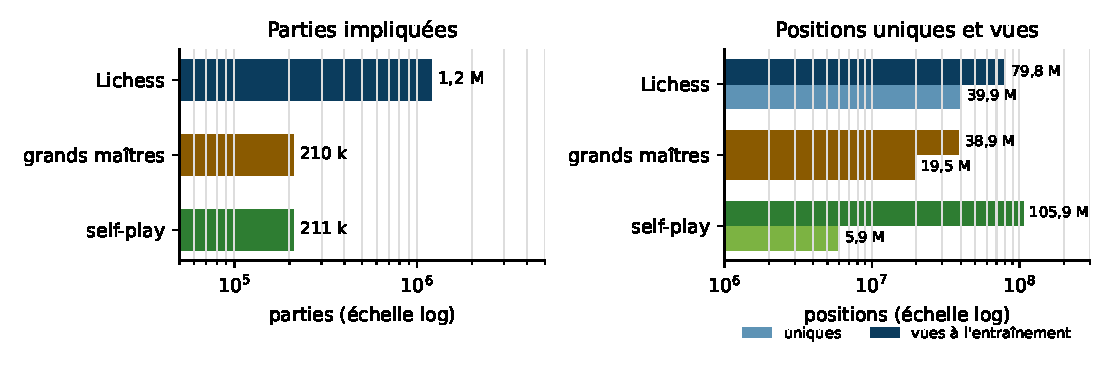
\includegraphics[width=\textwidth]{figures/fig_volumes.pdf}
\caption{À gauche, le nombre de parties par phase. À droite, les positions
uniques et le nombre de positions effectivement vues à l'entraînement
(échelle logarithmique). Pour le self-play, les positions « uniques » sont
les positions conservées, soit les coups joués sous recherche lente.}
\label{fig:volumes}
\end{figure}

\begin{table}[h]
\centering
\small
\caption{Récapitulatif des trois phases de la génération retenue.}
\label{tab:volumes}
\begin{tabular}{l r r r r}
\toprule
Phase & Parties & Positions uniques & Époques & Échantillons vus \\
\midrule
Lichess          & 1\,200\,000 & 39,9 M & 2  & 79,8 M \\
Grands maîtres   & 210\,000    & 19,5 M & 2  & 38,9 M \\
Self-play        & 211\,200    & 5,93 M & 18 & 105,9 M \\
\bottomrule
\end{tabular}
\end{table}

Le tableau~\ref{tab:volumes} et la figure~\ref{fig:volumes} racontent la même
histoire en deux temps. Les deux phases supervisées apportent l'essentiel de
la \emph{diversité} : 1,4 million de parties humaines, dont 39,9 M de positions
Lichess et 19,5 M de positions de grands maîtres, chacune parcourue deux fois.

\begin{chiffres}[Comment lire ces chiffres]
Une \emph{position unique} est une position stockée une fois dans un jeu de
données. Un \emph{échantillon vu} est une position présentée au réseau lors
d'un pas d'optimisation, c'est-à-dire une mise à jour des poids :
\[
\text{échantillons vus} = \text{steps} \times \text{taille de lot}.
\]
Un lot contient ici 2\,048 ou 4\,096 échantillons ; un échantillon n'est donc
pas un lot. Le nombre d'échantillons vus dépasse le nombre de positions
uniques dès que le même jeu de données est parcouru plusieurs fois, que ce
soit par époques multiples ou par rééchantillonnage du buffer. La vérification
est directe : $19\,495 \times 4\,096 = 79,8$ M pour Lichess et
$18\,996 \times 2\,048 = 38,9$ M pour les grands maîtres, soit deux époques
dans les deux cas.
\end{chiffres}

Le self-play, lui, n'apporte que 5,93 M de positions nouvelles, mais chaque
position est revue en moyenne 18 fois au fil des itérations. C'est la phase la
plus coûteuse en calcul pour le moins de données brutes, ce qui est le
principe même d'AlphaZero : la donnée est produite puis digérée en continu par
le modèle.

En cumulé, le modèle a vu 224,6 M de positions pendant son entraînement, dont
47 \% proviennent du self-play et 53 \% du supervisé. Le rapport entre les deux
mondes est un équilibre classique : assez de supervisé pour apprendre les
fondamentaux, assez de self-play pour dépasser la qualité des parties
humaines utilisées.

\begin{resume}
À retenir en trois points :
\begin{itemize}[leftmargin=1.1em,itemsep=1pt,topsep=2pt]
  \item le modèle est reparti de zéro le 6 avril, après avoir changé
        d'architecture (blocs SE) ; le transfert de poids testé ce soir-là a
        été abandonné à cause d'une tête de value inadaptée ;
  \item le supervisé apporte 1,4 M de parties humaines et 59,4 M de positions
        uniques ; le self-play ajoute 211\,000 parties et 5,93 M de positions,
        revues 18 fois en moyenne ;
  \item en 23 jours, le niveau estimé passe d'environ 2\,490 à environ
        2\,650 Elo, avec un pic à 2\,892 face à Stockfish 2\,600.
\end{itemize}
\end{resume}
